\chapter{Convenções de nomenclatura e definições}

\section{Modelo de Domínio}

\begin{figure}[!htb]
\centering
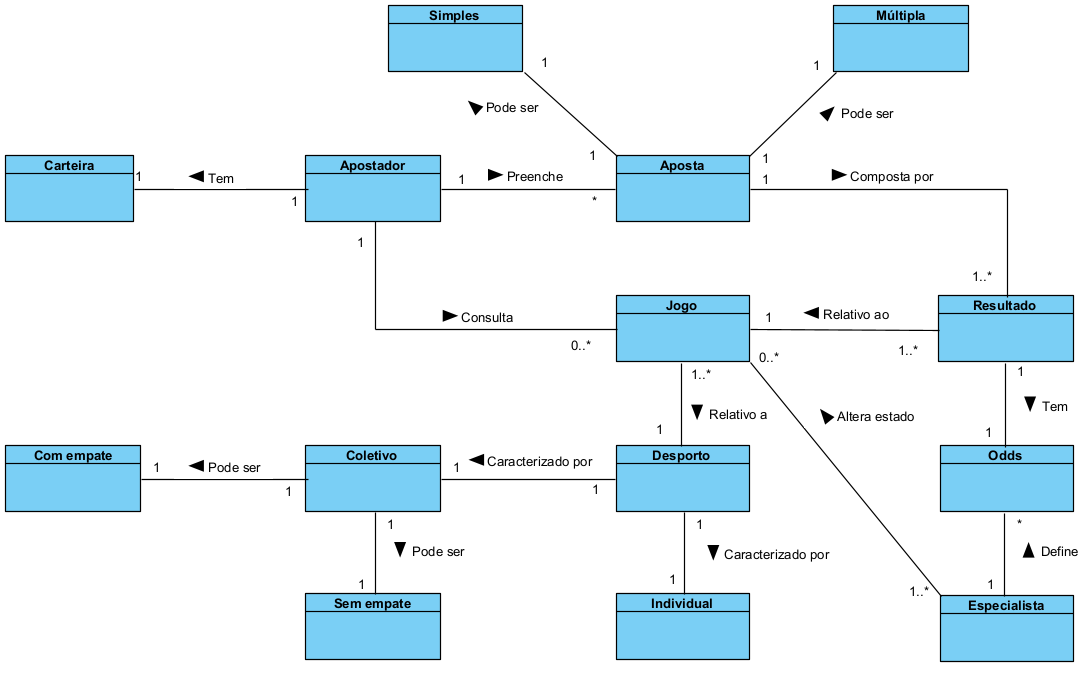
\includegraphics[width=1\linewidth]{imagens/convencao/domainModel.png}
\caption{Modelo de Domínio }
\label{}
\end{figure}%

\section{Definição de entidades}

Nesta secção, são abordadas as diferentes entidades presentes no Modelo de Domínio apresentado na secção anterior (figura 5.1). 

\begin{itemize}
    \item \textbf{Apostador:} Principal utilizador do sistema, cujo proveito da aplicação é tirado por este, na medida em que é o usufruidor da aplicação;
    \item \textbf{Especialista:} Utilizador encarregue das \textit{odds};
    \item \textbf{Administrador:}  Utilizador responsável pela alteração do estado da aposta, ou seja, se esta está ativa, fechada, ou suspensa. Este também é responsável pela gestão de notificações e criação de promoções.
    \item \textbf{Carteira:} O Apostador tem uma carteira que guarda o dinheiro que transfere para o \textit{web site} e ganha das apostas;
    \item \textbf{Jogo:} O apostador pode consultar a listagem de jogos, entre os desportos disponíveis. Cada jogo tem resultados disponíveis para seleção/aposta;
    \item \textbf{Aposta:} É a principal atividade e funcionalidade do \textit{site} de apostas. Esta é composta por resultado(s) de jogo(s), podendo ser simples ou múltipla, consoante o número de resultados de jogos diferentes selecionados; 
    \item \textbf{Aposta Simples:} Uma aposta simples contém apenas 1 resultado (Vitória da equipa 1, Empate ou Vitória da equipa 2) de um jogo, o qual deverá ser vencedor para que a sua aposta seja ganha. Os retornos possíveis são calculados multiplicando o valor da sua aposta pela \textit{odd} disponibilizada;
    \item \textbf{Aposta múltipla:} Uma aposta múltipla contém 2 ou mais resultados de jogos diferentes, em que todos terão de ser vencedores para que a aposta seja ganha. O conceito de "multiplicador" é aplicado para o cálculo das \textit{odds} totais do boletim de apostas e, consequentemente, aos seus potenciais ganhos. Estes são calculados multiplicando o valor da sua aposta pelo produto das várias \textit{odds} no boletim de apostas;
    \item \textbf{\textit{Odd}:}  As \textit{Odds} são cotações dadas a determinado jogo, ou seja, de forma simples elas designam as probabilidades de um determinado evento ocorrer;
    \item \textbf{Desporto:} Modalidades disponíveis no RASBet;
    \item \textbf{Desporto Individual:} O desporto individual é  praticado por cada pessoa, separadamente;
    \item \textbf{Desporto Coletivo:} Desporto coletivo são desportos praticados por duas ou mais pessoas;
    \item \textbf{Desporto Coletivo com Empate:} Desporto coletivo com empate são desportos praticados por duas ou mais pessoas, cujo o "Empate" é opção de resultado, ou seja, do formato V1 | X | V2. 
    \item \textbf{Desporto Coletivo sem Empate:} Desporto coletivo sem empate são desportos praticados por duas ou mais pessoas, cujo o "Empate" não é opção de resultado.
    
    \item \textbf{Resultado:} Representa os resultados de jogos, que o apostador pode selecionar/apostar. No caso de ser um jogo de desporto coletivo com empate, este pode selecionar entre os resultados V1, X e V2, no caso de ser um jogo de desporto coletivo sem empate, só pode selecionar entre os resultados V1 e V2. O apostador, numa mesma aposta, só pode selecionar um dos resultados disponíveis em cada jogo consultado, seja numa aposta simples ou múltipla. 
      
    \item \textbf{Notificações:} Notificações do sistema que anunciam o resultado das apostas quando um jogo acaba, e promoções criadas pelo administrador.
\end{itemize}